\section{Illumination et éclairement}

\begin{frame}{De la lumière à la couleur}
\begin{itemize}
\item Modèle d'éclairement : \textit{OpenGL}
\item Ombrages
\item Elimination des parties cachées
\item Textures
\item Aliassage (aliasing)
\end{itemize}
\end{frame}


\begin{frame}{Illumination : le modèle d'OpenGL}
\begin{itemize}
\item Modèle précis d'éclairement : intégration des modèles optiques et quantiques
\item Un modèle qui fait pas mal d'hypothèses restrictives
\item Les objets sont éclairés, ils renvoient tout ou partie de la lumière venant des sources lumineuses
\item On exclut toute interaction entre les objets
\begin{itemize}
\item Pas d'ombres, pas de reflets, pas de transferts de couleurs...
\item \textbf{Objectif} : calculer la couleur des objets en tout point de leur surface
\end{itemize}
\end{itemize}
\end{frame}

\begin{frame}[t]{Le modèle d'OpenGL}
  \begin{itemize}
    \item 4 composantes lumineuses
    \begin{itemize}
      \item la composante \textbf{émissive}
      \item la composante \textbf{ambiante}
      \item la composante \textbf{diffuse}
      \item la composante \textbf{spéculaire}
    \end{itemize}
    \item 4 types de sources de lumière
  \end{itemize}
\end{frame}
%--- Next Frame ---%
%--- Next Frame ---%

\begin{frame}[t]{Source ponctuelle}
  \begin{itemize}
    \item Isotrope
    \item atténuation (éventuelle) en fonction de la distance
  \end{itemize}
    \begin{center}
      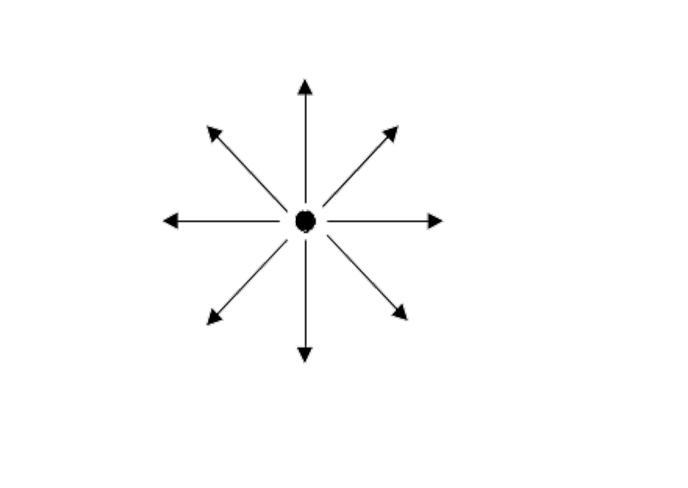
\includegraphics[height=5cm]{figs/src-ponctuelle.pdf}
      \end{center}
\end{frame}
%--- Next Frame ---%

\begin{frame}[t]{Source directionnelle}
  \begin{itemize}
    \item Modèle : soleil, suffisamment gros par rapport à l'objet d'intérêt pour que tous les rayons paraissent parallèles
    \item sous entendu : une seule par scène
  \end{itemize}
    \begin{center}
      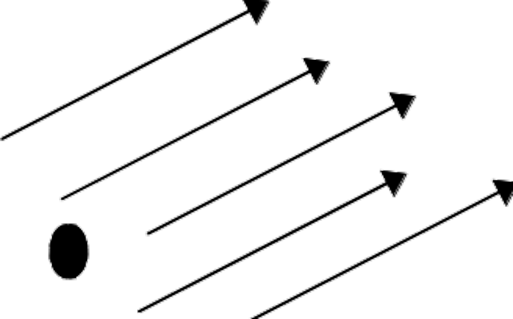
\includegraphics[height=4cm]{figs/src-dir.pdf}
      \end{center}
\end{frame}
%--- Next Frame ---%

\begin{frame}[t]{Source de type spot}
  \begin{itemize}
    \item Une direction privilégiée d'éclairage
    \item Atténuation en fonction de
    \begin{itemize}
      \item distance à l'origine
      \item angle par raport à l'axe
    \end{itemize}
  \end{itemize}
    \begin{center}
      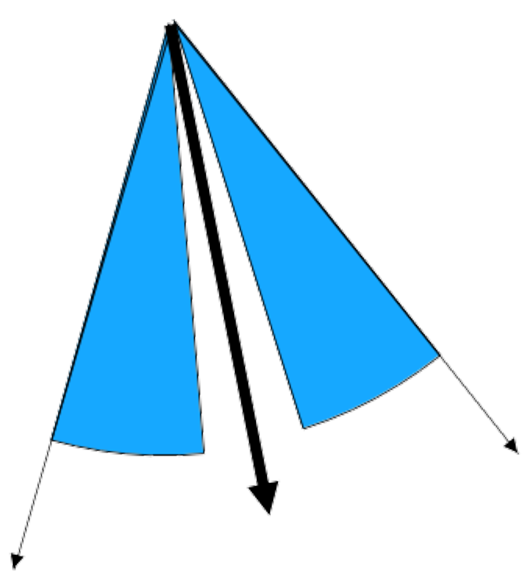
\includegraphics[height=5cm]{figs/src-spot.pdf}
      \end{center}
\end{frame}
%--- Next Frame ---%

\begin{frame}[t]{Eclairage ambiant}
  \begin{itemize}
    \item Isotrope
    \item Uniforme
  \end{itemize}
    \begin{center}
      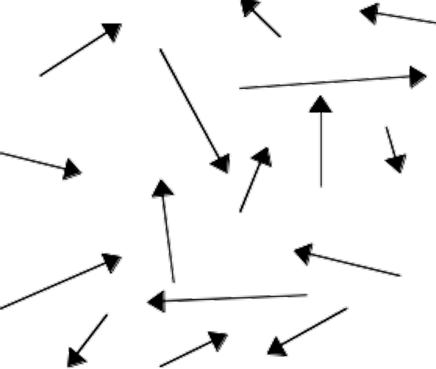
\includegraphics[height=5cm]{figs/src-ambiant.pdf}
      \end{center}
\end{frame}
%--- Next Frame ---%

\begin{frame}[t]{Réflexion ambiante}
  \begin{itemize}
    \item La couleur ne dépend pas de la position, uniquement de l'objet : $I = I_a K_a$
    \begin{itemize}
      \item $I_a$ : lumière ambiante
      \item $K_a$ : coefficient de réflexion ambiante
    \end{itemize}
    \item Modèle très primitif
    \begin{itemize}
      \item Pas de sens physique possible
      \item La forme des objets est invisible
      \item Néanmoins très utile pour masquer les autres défauts du modèle...
    \end{itemize}
  \end{itemize}
\end{frame}
%--- Next Frame ---%

\begin{frame}[t]{Intensité ambiante}
$$I = I_a K_a$$
\begin{center}
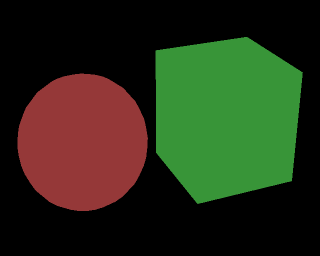
\includegraphics[width=.3\textwidth]{figs/amb1.png} \\
\end{center}

\begin{center}
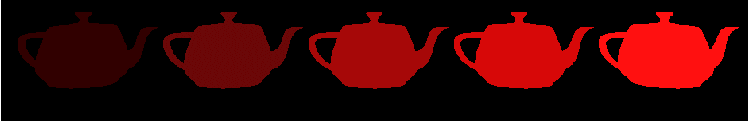
\includegraphics[height=2cm]{figs/amb2.png}
\end{center}

\end{frame}
%--- Next Frame ---%

\begin{frame}[t]{Modèle de Phong}
  $$ I_r = I_a + I_d + I_s $$
  \begin{itemize}
    \item $I_r$ : intensité réfléchie
    \item $I_a$ : intensité ambiante
    \item $I_d$ : intensité diffuse (uniforme)
    \item $I_s$ : intensité spéculaire (réflexion parfaite)
  \end{itemize}
  \begin{center}
  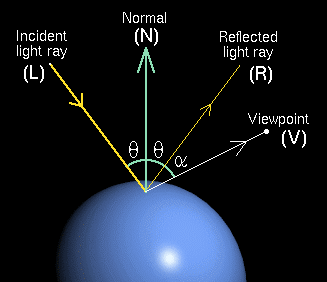
\includegraphics[height=3.5cm]{figs/normals.png}
  \end{center}

\end{frame}
%--- Next Frame ---%

\begin{frame}[t]{Réflexion diffuse}
  \begin{center}
    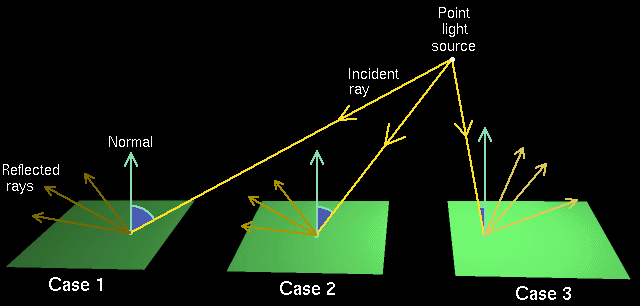
\includegraphics[height=6cm]{figs/diffuse.png}
  \end{center}
\end{frame}
%--- Next Frame ---%

\begin{frame}[t]{Intensité diffuse}
  $$ I_d = K_d \sum_j < N | L_j > I_{obj} I_j $$
  \begin{itemize}
    \item Loi de Lambert
      \begin{itemize}
        \item $K_d$ : coefficient de diffusion de la surface
        \item $N$ : normale à la surface
        \item $L_j$ : direction du rayon incident
        \item $I_{obj}$ : "couleur" de l'objet
        \item $I_j$ : "couleur" de la source lumineuse
      \end{itemize}
  \end{itemize}
\end{frame}
%--- Next Frame ---%

\begin{frame}[t]{Réflexion spéculaire}
  \begin{columns}
    \begin{column}{.49\textwidth}
      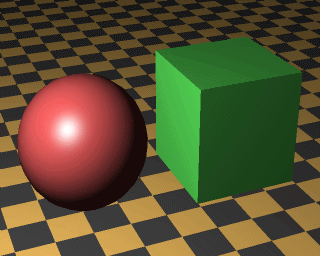
\includegraphics[width=\textwidth]{figs/spec1.png} \\
      Pas uniquement ponctuelle
    \end{column}
    \begin{column}{.49\textwidth}
      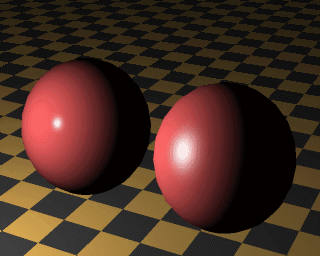
\includegraphics[width=\textwidth]{figs/spec2.png} \\
      Dépend du matériau considéré
    \end{column}
  \end{columns}
\end{frame}
%--- Next Frame ---%

\begin{frame}[t]{Intensité spéculaire}
  $$ I_s = \sum_j K_s(j) < R_j | V >^n I_j $$
  \begin{columns}
    \begin{column}{.59\textwidth}
      \begin{itemize}
        \item $K_s$ : constante de spécularité
        \item $R_j$ : rayon réfléchi
        \item $V$ : vecteur objet-caméra
        \item $n$ : dépend du type de matériau
      \end{itemize}
    \end{column}
    \begin{column}{.39\textwidth}
      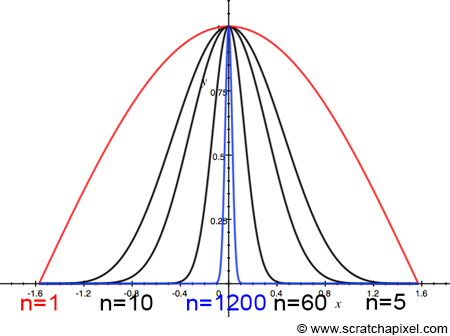
\includegraphics[width=\textwidth]{figs/cosn.png} \\

    \end{column}
  \end{columns}
\end{frame}
%--- Next Frame ---%

\begin{frame}[t]{Variation de la réflexion spéculaire}
  \begin{center}
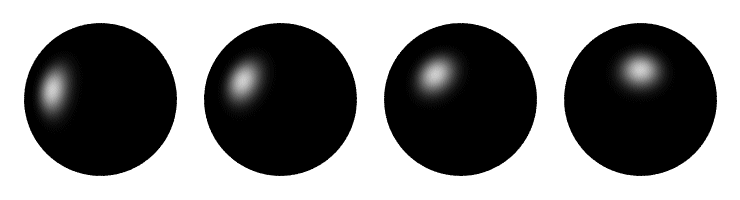
\includegraphics[height=2.5cm]{figs/spec3.png} \\
Si on déplace la source  lumineuse
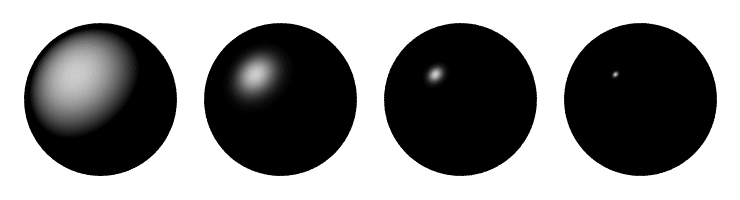
\includegraphics[height=2.5cm]{figs/spec4.png} \\
Si on change la brillance du matériau

  \end{center}
\end{frame}
%--- Next Frame ---%
\begin{frame}[t]{Divers}
  \begin{itemize}
    \item Atténuation des sources lumineuses
    \begin{itemize}
      \item plusieurs modèles possibles
      \item $I_{att} = F_{att} I_d$ où $F_{att} = \frac{1}{D_l^2}$ ou $F_{att} = \min \left( \frac{1}{c_1+c_2D_l+C_3D_l^2},1 \right) $
      \item $D_l$ = distance à la source lumineuse
      \item Note : on peut aussi simuler l'atténuation atmosphérique en prenant aussi en compte la distance à l'observateur
    \end{itemize}
    \item Transparence (simpliste) : $I = K_tI_r + (1-K_t)I_{back} $
  \end{itemize}
\end{frame}
%--- Next Frame ---%
